% Document downloaded from http://overleaf.com
\documentclass[format=acmsmall]{acmart}
\usepackage[utf8]{inputenc}
\usepackage{graphicx}

\AtBeginDocument{%
  \providecommand\BibTeX{{%
    \normalfont B\kern-0.5em{\scshape i\kern-0.25em b}\kern-0.8em\TeX}}}

\setcopyright{acmcopyright}

% Package config
\graphicspath{ {./images/} }
\bibliographystyle{ACM-Reference-Format}

\begin{document}

% Metadata
\title{Facilitating the achievement of flow by using an IoT device for reducing smartphone checking habits}
\keywords{iot, arduino, smartphone checking, habits, flow}
\author{João Lúcio Gomes}
\affiliation{%
    \institution{Rhine-Waal University of Applied Sciences}
    \streetaddress{Friedrich-Heinrich-Allee 25}
    \city{Kamp-Lintfort}
    \state{North Rhine-Westphalia}
    \country{Germany}
    \postcode{47475}
}
\email{joao-lucio.martins-ferreira-gomes@hsrw.org}
\date{February 2021}

\begin{abstract}
Smartphone checking habits introduce interruptions that interfere with individuals' attainment of flow, a mental state characterized by deep focus and intrinsic motivation when performing work. This paper tests the viability of an experimental IoT-enabled device as a means for disrupting the checking habit and aiding users in achieving flow-like states. Analysis from data collected by a Work-Related Flow Inventory (WOLF) questionnaire showed no difference in the incidence of flow when using the device. Nevertheless, comparison of means and a semi-structured interview point towards the device helping users attain better focus, suggesting a second iteration of the product could function as a flow facilitator by employing a different reward strategy.
\end{abstract}

\begin{CCSXML}
<ccs2012>
   <concept>
       <concept_id>10003120.10003121.10003125</concept_id>
       <concept_desc>Human-centered computing~Interaction devices</concept_desc>
       <concept_significance>300</concept_significance>
       </concept>
   <concept>
       <concept_id>10003120.10003121.10003122.10003334</concept_id>
       <concept_desc>Human-centered computing~User studies</concept_desc>
       <concept_significance>500</concept_significance>
       </concept>
 </ccs2012>
\end{CCSXML}

\ccsdesc[300]{Human-centered computing~Interaction devices}
\ccsdesc[500]{Human-centered computing~User studies}

\maketitle
 
\section{Introduction}

In a study recently performed in Germany among adult, working people who own a smartphone ($N=262$), it has been detected that smartphone-induced interruptions in the workplace have a negative relationship with users' self-assessed levels of productivity \cite{duke_montag_2017}. It highlighted the fact that users may develop a so-called \textit{checking habit} \cite{oulasvirta_rattenbury_ma_raita_2011}, which leads to interruptions, hence preventing users from achieving \textit{flow}: a mental state characterized by high levels of focus, creativity and satisfaction.

Several products\cite{biber}\cite{amazon_01}\cite{amazon_02} and techniques exist that encourage people to leave their devices aside (the Pomodoro technique\cite{cirillo_2018} is very popular), but no product exists for fostering the construction of an actual habit of keeping the smartphone at bay and helping with the attainment of flow, as none of them offer extrinsic rewards.

Our hypothesis is that we can disrupt the checking habit and promote the achievement of flow-like states in users. We propose an experimental device that suppresses the habit's cues, replaces its routine and offers a reward for not interacting with the device for extended periods of time. 

\section{The Checking Habit \& The Flow State}

Habits are automatic behavior cycles, comprised of a \textit{cue}, a \textit{routine} and a \textit{reward}. Individuals anecdotally perceive the routine as being the habit, but the whole cycle has to be taken into consideration when discussing this subject. The routine is merely one of the components, and the means for one to achieve a goal --- the reward \cite{duhigg_2014}.

The checking habit specifically is cued by context: just having the smartphone in sight is enough to trigger one's routine of waking the device up. This is reinforced by the fast and easy-to-use nature of the smartphone, and one's anticipation for interacting with reward-driven content therein \cite{oulasvirta_rattenbury_ma_raita_2011}. Having the device visible and within reach is linked to higher levels of inattention and a higher number of interruptions, regardless of whether the device is in Silent or Do Not Disturb modes. \cite{kushlev_proulx_dunn_2016}. 

Furthermore, flow is an autotelic "hyper-focused" mental state where one is fully immersed in an activity. Two requirements must be met to achieve this state: there has to be a match between one's skill and the performed task, and there should be several minutes of uninterrupted focus \cite{csikszentmihalyi_1990}. In the context of professional tasks, flow is characterized by feelings of intrinsic work motivation, work enjoyment and full absorption \cite{bakker_2005}. Given that individuals report feeling happier, more focused, more creative, and more satisfied with their activities in flow-like states \cite{csikszentmihalyi_lefevre_1989}, it is easy to see why achieving them is desirable, and why interruptions caused by smartphones can be detrimental to fulfilling that goal.

\section{Experiment}

\subsection{Experimental Design}

A repeated-measures study was selected, where the independent variable is the occurrence of flow-like states on the participants. Counterbalancing was used to account for eventual order effects.

\subsection{Testing Material}

\begin{figure}
    \centering
    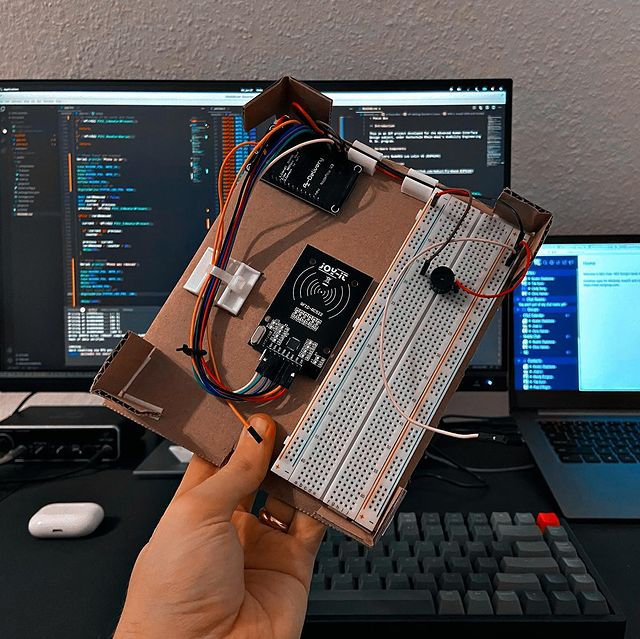
\includegraphics[height=7cm]{box_1}
    \caption{The box's interior, with ESP8266, MFRC522 and connections visible.}
    \label{fig:box_1}
\end{figure}

A prototype was built using a simple cardboard box, an \texttt{ESP8266} micro-controller board and an \texttt{MFRC522} NFC card reader (As seen in Figure \ref{fig:box_1}). It also employs a web application devised to yield friendly feedback and produce a reward --- keeping a persistent record of the amount of time spent not interacting with the smartphone.\footnote{The project's source code is available on https://github.com/uxbyjoao/focus-box. This URL also includes a link to a video demonstrating the device's usage.}

The box continually checks for the presence of an RFID card, and triggers server-side code to track the amount of time the card remained inside it. RFID cards are then glued to the back of participants' smartphones, so that the smartphone triggers the RFID logic when inside the box.

\subsection{Participants}

Participants were selected based on their occupation and current work arrangements. It was required that they:
\begin{enumerate}
    \item Own a smartphone
    \item Perform work in long sessions while sitting down at the computer
    \item Are currently employed and working from home
\end{enumerate}

Based on this criteria, three participants volunteered: one male graphic designer (33), one male government employee (32), and one female photographer (28).

\subsection{Tasks}

Users were each asked to perform two one-hour work sessions, carrying out normal tasks that they usually perform for their jobs: one session with their smartphones in plain view, within reach, and the other with their smartphones inside the box.

\subsection{Measurement}

Measurement of flow was made using the Work-Related Flow Inventory, or WOLF \cite{bakker_2008}. It employs a 7-point Likert scale and measures the following dimensions to flow: absorption (4 items), work enjoyment (4 items) and intrinsic work motivation (5 points).

The questionnaire was, in this instance, modified for verb tenses i.e. the original questionnaire uses present tense verbs. We also employed a 5-point Likert scale instead of a 7-point for the sake of simplicity.

Participants were also asked to take part in a short semi-structured interview for assessing their general feelings towards smartphone interruptions, the device and its utility. It consisted of three open-ended questions:

\begin{enumerate}
    \item Do you feel like your smartphone sometimes prevents you from staying focused at work?
    \item Did using the focus box help you in suppressing any interruptions from your smartphone in any way?
    \item Would you be interested in using such a device as a part of your daily working routine?
\end{enumerate}

\subsection{Procedure}

The experiment was performed at each participant's home. Due to COVID-19, social distancing rules were mutually established and enforced.

An explanation of the system was given, along with instructions regarding the requirements for each work session. After finishing the sessions, each participant was asked to fill out a WOLF questionnaire, filling out two in total --- one for the phone in the box, one for the phone outside the box. Following the two sessions, they were invited to participate in the interview.

No instructions or requirements were made as to whether participants could or could not remove the smartphone from the box during the task where the former was supposed to be inside the latter. Participants were explicitly told they were free to interact with the smartphone if they pleased at any point during both work sessions.

To avoid demand characteristics, participants were left alone in a separate room during the work sessions. 

\section{Results}

All three subjects completed all the experiment's tasks successfully.

A Mann-Whitney U test was applied to the data collected from the FLOW questionnaire, per participant. The results of this test were combined with the means for each scenario for analysis. This data is available on Table \ref{tab:results}. 

The p-value was $>0.05$ for all three participants, therefore confirming the null hypothesis.

Semi-structured interview results were mostly positive, where 2 out of 3 participants reported that using the box helped them avoid interruptions from their smartphones during their work. Only one participant reported that they would use the device in day-to-day work activities.

\begin{table}[ht]
\centering
\begin{tabular}{|l||cc||cc|}
\hline
 & z-score & p-value & Mean (outside) & Mean (inside) \\ \hline
Participant A & -0.051 & 0.480 & 2.76 & 2.84 \\
Participant B & -1.076 & 0.140 & 4.07 & 4.46 \\
Participant C & -0.692 & 0.245 & 2.61 & 2.84 \\ \hline
\end{tabular}
\caption{Mann-Whitney U test applied to WOLF data, combined with means.}
\label{tab:results}
\end{table}

\section{Discussion}

We found no absolute difference in incidence of flow by using the box when analyzing p-values alone. However, upon interviewed, participants reported that the box indeed helped them when avoiding interruptions caused by the smarpthones. This is confirmed by comparing the means between scenarios in Table \ref{tab:results}. It suggests that using the box is more of a "nudge" towards not checking the phone than a full-on deterrent against the checking habit.

This "nudging" is clear from one of the participant's interview responses: he reported that having the phone inside the box gave him the impression that it was "under arrest" for a while and off limits to him, which made him make a conscious effort to not touch it for a while. This participant felt the box helped him focus, and would use it on a daily basis.

From the interview, we could see that the concept was interesting to participants, although one of them said that it would be more of a nuisance than a utility. The reason given is they do not feel smartphone interruptions are that much of a problem in a work environment. This was expected, and has already been detected in previous research \cite{oulasvirta_rattenbury_ma_raita_2011}.

It is also possible that users simply do not value the reward offered by the experimental device as previously anticipated. Therefore, an iteration of the device could be built employing a different reward for staying away from the device. One possible avenue worth exploring, which has been shown to be successful in habit forming, is gamification \cite{robson_plangger_kietzmann_mccarthy_pitt_2015}.

Overall, a study where more users perform longer work sessions over a period of days instead of hours would inexorably yield better data for evaluation. The Mann-Whitney U test yields better results when the sample size is $>10$. This study was carried out while lockdown measures were in place in Germany due to the COVID-19 outbreak --- the circumstances therefore dictated its duration and sample size.

\bibliography{bibliography}

\end{document}
